\chapter{Анализ задачи}

\section{Обзор существующих реализаций палитр команд}\label{analogs}

Впервые палитра команд появилась 1 июля 2011 году в редакторе Sublime Text
2~\cite{sublimetext2changelog}. Вслед за этим подобная функция была реализована
в некоторых других программах. Таких, как:
\begin{itemize}
	\item Atom\cite{atom},
	\item VSCode\cite{vscode},
	\item JupyterLab\cite{jupyterlab}.
\end{itemize}

Но это были лишь единичные случаи. В апреле 2017 года появилась альфа-версия
приложения Plotinus\cite{plotinus}, которое позволяет добавлять палитру команд в
любое приложение, использующее графическую библиотеку GTK.

Таким образом можно наблюдать, что частные решения начинают заменяться более
универсальными. Однако на текущий момент эти решения не позволяют покрыть
большинство областей т.к. ограничены лишь программами с GTK, который
используется не более чем в половине прикладных приложений для ОС Linux и
занимает совсем малую долю среди приложений для ОС Windows.

\begin{figure}[h]
	\centering
	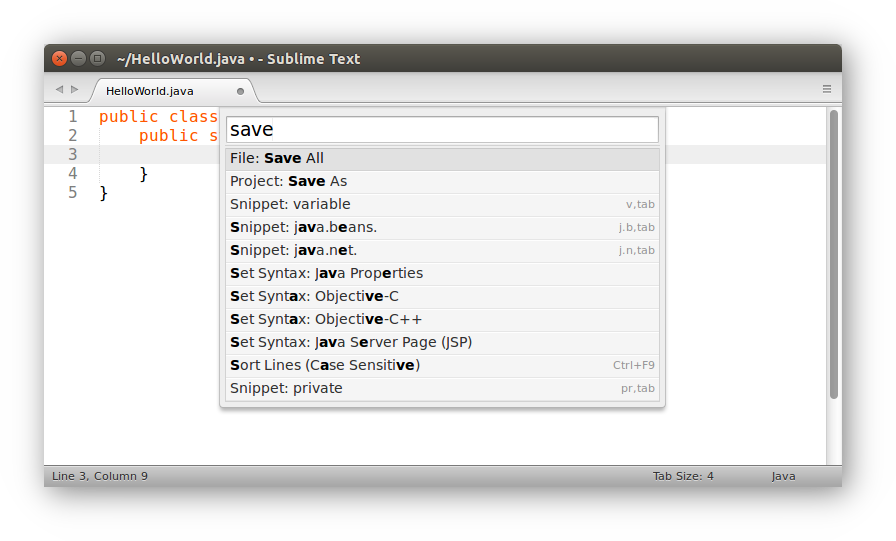
\includegraphics[width=0.9\textwidth]{SublimeText}
	\label{sublimetext}
	\caption{Sublime Text}
\end{figure}

\begin{figure}[h]
	\centering
	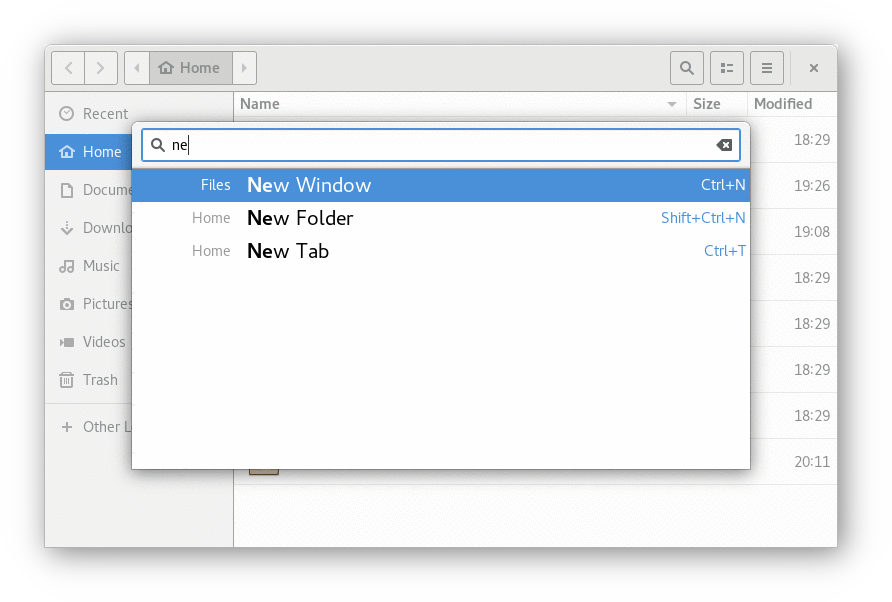
\includegraphics[width=\textwidth]{Plotinus}
	\caption{Plotinus}
\end{figure}

\section{О фреймворке Qt}

Qt — это кроссплатформенный фреймворк для разработки программного обеспечения
на языке программирования C++\cite{qtabout}. Он содержит множество библиотек для
упрощения реализации прикладных задач. Благодаря кроссплатформенности данный
фреймворк позволяет запускать написанное с его помощью ПО на многих операционных
системах путем обычной сборки проекта без внесения изменений в исходный код
самой программы. Отличительной особенностью Qt является наличие метаобъектного
компилятора, который запускается в начале сборки и генерирует
вспомогательный код. Такой подход позволил добавить частичную поддержку
рефлексии.

Qt включает в себя следующие модули:

\begin{itemize}
    \item Qt Core — базовые классы, обеспечивающие рефлексию, работу со
        строками, механизмы владения и т.п. Используются всеми остальными
        модулями;
    \item Qt Network — классы, позволяющие легко писать переносимый код для
        работы с сетью;
    \item Qt SQL — классы, предоставляющие удобный программный интерфейс для
        работы с различными реляционными БД;
    \item Qt Multimedia — классы, для работы с данными (аудио и видео),
        устройствами (камеры, микрофоны);
    \item Qt GUI — классы, позволяющие реализовать приложения с графическим
        интерфейсом.
\end{itemize}

В ОС Linux библиотеки GTK и Qt являются двумя наиболее популярными средствами
для реализации приложений с графическим интерфейсом. Т.к. средство для
добавления палитры команд уже есть для GTK, в данной работе будет рассмотрена
такая возможность для Qt.

События в Qt — это объекты, унаследованные от абстрактного класса \code{QEvent}.
Они представляют действия, произошедшие внутри приложения, либо созданные в
результате активности пользователя, о которых приложение должно знать. События
могут быть получены и обработаны любым экземпляром подкласса \code{QObject}, но
они особенно актуальны для графических элементов.

Обычно события доставляются объектам через вызов виртуальных функций. Если
разработчик хочет заменить функцию базового класса, он должен реализовать
всю обработку самостоятельно. Однако, если нужно только расширить
функциональность то разработчик должен реализовать нужное расширение, а затем
вызывать базовый класс, чтобы обеспечить поведение по умолчанию для тех случаев,
которые он не хочет обрабатывать.

Не всегда в классе имеется нужная функция для события. Наиболее распространенный
пример — обработка нажатия клавиш, для которой нет соответствующей виртуальной
функции. Для обработки таких событий нужно переопределить метод
\code{QObject::event()}. Он является общим обработчиком событий, и позволяет
выполнить дополнительные действия до или после обработки по-умолчанию.

\section{Организация работы приложения}

Система управления должна позволять контролировать множество приложений. Для ее
реализации лучше всего подходит клиент-серверная архитектура. Для каждого
целевого приложения запускается отдельный клиент, который занимается сбором
информации об элементах управления и передает ее на сервер.

В качестве сервера будет выступать приложение, которое запускает целевые
приложения вместе с клиентами. После этого сервер принимает входящее соединение
от клиента и отображающее окно поиска элемента для текущего активного окна.

Для удобной работы окно поиска должно отображаться окно поверх текущего
активного приложения. Палитра команд является инструментом для помощи
пользователю в поиске нужной функции. Он может не знать точное наименование
команды, поэтому в приложении должна быть поддержка нечеткого поиска.

\subsection{Добавление логики в стороннее приложение}

Разработчики любого приложения не могут учесть желания и капризы всех
пользователей. Благодаря этому приложения не превращаются в комбайны, которые
невозможно было бы поддерживать. Разработчики могут убрать какую-то деталь,
которая нужна малому проценту людей. Ведь надо тратить время на исправление
ошибок в ней. А иногда эти специфичные функции могут даже замедлять работу всего
приложения. В таком случае пользователи могут захотеть добавить какую-то
дополнительную логику или функцию в основное приложение.

Подходы делятся на два типа:
\begin{itemize}
	\item добавление функции на этапе сборки приложения;
	\item добавление функции в момент выполнения программы.
\end{itemize}

Целью данной работы является добавление функциональности в максимальную группу
приложений. Первый же подход исключает такую возможность для приложений с
закрытым исходным кодом. К тому же при первым подходом может пользоваться только
квалифицированный пользователь. И то, ему пришлось бы пересобирать каждое
приложение в которое он хотел бы добавить нужную функциональность.

Программный модуль подключаемый к уже существующему приложению называется
плагином. Для добавления возможности их подключения разработчики программы
должны или написать свою систему плагинов или воспользоваться готовой. Так,
например, библиотека GTK, начиная с третьей версии, предоставляет возможность
запускать приложения с дополнительными модулями, которые могут расширять
функциональность приложения. Этим воспользовались разработчики библиотеки
Plotinus, реализовав возможность добавления палитры команд в любое приложение,
использующее GTK.

Qt предоставляет возможность встраивать дополнительную функциональность в
приложение, но для этого оно должно иметь специальный код по загрузке
дополнительных модулей, который в большинстве случаев не используется (для
подтверждения можно сравнить число github репозиториев использующих
Qt\cite{githubqt} и использующих функцию Qt для работы с
плагинами\cite{githubqpluginloader}. Соотношение примерно 1:100).

Кроме штатных средств добавления возможностей на уровне приложения есть и более
низкоуровневые. Так например в Windows есть функция автоматизации интерфейса: UI
Automation\cite{windowsuiautomation}, которая изначально была добавлена для
увеличения доступности приложений людям с ограниченными возможностями. С её
помощью можно работать только с видимыми элементами интерфейса, но не получать
внутренние состояния (что можно сделать через плагины), но зато доступен для
любого приложения, использующего стандартные элементы управления. В случае
использования Linux, к сожалению, нет такой возможности на уровне ОС или
графической оболочки.

\subsection{Внедрение модуля}

Рассмотрим в общих чертах механизм работы графического приложения. На
рисунке~\ref{fig:gui} изображено как происходит взаимодействие между элементами
графического приложения и пользователем.

\begin{figure}
	\centering
	\begin{tikzpicture}[
        ->,>=stealth',node
        distance=1.5cm, semithick,
        every edge/.append style={<->}
    ]

    \tikzstyle{block} = [rectangle,draw,minimum height=0.8cm]

    \node[block] (user) {Пользователь};
    \node[block] (x11) [below of=user] {Графическая подсистема X11};
    \node[block] (lib) [below of=x11] {Графическая библиотека Qt};
    \node[block] (app) [below of=lib] {Приложение};
    \path[]
        (user) edge (x11)
        (x11) edge (lib)
        (lib)  edge (app)
    ;

\end{tikzpicture}
\\
	\caption{Взаимодействие элементов ГИП и пользователя}\label{fig:gui}
\end{figure}

Исходя из данной упрощенной схемы можно предложить еще одно способ добавить
функциональность — создание события от графической библиотеки, которое будет
передано приложению.

\subsection{Механизм подмены функций}

При запуске приложения загрузчик получает из него список всех используемых
динамических библиотек, загружает их в память. Затем получает адреса всех
экспортированных функций динамической библиотеки и сохраняет их для последующего
вызова.

Загрузчик ld, который используется в Linux и FreeBSD позволяет загружать
дополнительные динамические библиотеки, кроме тех, кто запрашивает приложение.
Эта дополнительная библиотека загружается раньше всех остальных, что позволяет
ей подменять функции из других библиотек. Это происходит потому, что при поиске
адреса определенной функции берется первый подходящий.

\subsection{Способ получения информации об элементах}

Для получения информации об элементах интерфейса можно загрузить специальную
библиотеку, которая будет регистрировать создания, изменения и удаления
элементов интерфейса. Затем собранная информация будет передавать на сервер для
последующей работы.

Также данная библиотека может создавать ложные события по командам, приходящим с
сервера. Таким образом можно имитировать нажатия кнопок, открытие меню и т.п.

Пользовательский интерфейс через специальное API сможет получать от сервера
информацию о доступных элементах в текущем приложении. После того, как
пользователь произвел выбор, вызывается специальная функция на стороне сервера,
которая приводит к отправке команды клиенту.

\subsection{Реализация кода для подмены функции}

Для внедрения библиотеки требуется реализовать заглушки функций Qt, которые
будут вызывать специальный обработчик, а затем продолжать нормальное выполнение
функции. Дополнительную сложность создает то, что библиотека Qt написана на
языке C++, который из-за поддержки классов и перегрузок функций использует т.н.
«искажение имен» (name mangling). Таким образом, чтобы создать обработчик,
нужно сконструировать специальное имя функции исходя из названия класса,
метода, набора параметров и возвращаемого значения.

Создание таких обработчиков является рутинной задачей в которой человек легко
может допустить ошибку. Поэтому вместо ручного написания каждого обработчика
нужно написать генератор, который может добавить необходимые обработчики, имея
минимальный и необходимый набор данных (имя класса, метода и т.д.).

\subsection{Требующиеся компоненты}

Исходя из приведенного выше анализа следует, что задачи должны быть сгруппированы
в набор программ. Он должен быть реализован в виде следующих элементов:

\begin{enumerate}
	\item\label{lib} Библиотека для внедрения и сбора информации в приложении.
	\item Приложение для сохранения информации, полученной из нескольких
	приложения с библиотекой из пункта \ref{lib}.
	\item Интерфейс для запуска приложений и отображения палитры команд.
\end{enumerate}

\section{Архитектура системы}

Подходящая архитектура для такой задачи была предложена в
работе\cite{polshakovinject}. Вся система может быть разделена на три основные
части:

\begin{enumerate}
    \item регистрация изменений в элементах приложения;
    \item посылка команды;
    \item активация элемента.
\end{enumerate}

Рассмотрим детально каждую из них.

\subsection{Регистрация нового элемента}

При запуске приложения, в него внедряется подгружаемый модуль, который
переопределяет некоторые функции библиотеки Qt. Благодаря механизму работы
загрузчика, целевое приложение будет на самом деле вызывать поддельные
функции, вместо реальных.

Когда приложение создает элемент интерфейса или меняет описание уже
существующего происходит вызов соответствующей функции, которую мы
перехватываем. После этого наша библиотека посылает на сервер информацию
о новом элементе или об изменении старого.

Когда все дополнительные действия сделаны, библиотека должны обеспечить
стандартное поведение функции, которую она подменила. Для этого, используя
механизмы загрузчика, она получает адрес настоящей функции и передает
управление Qt. Графическая библиотека в свою очередь занимается формированием
изображения и передает его на отрисовку в графическую подсистему X11.

На рисунке~\ref{fig:create-elem} изображена диаграмма последовательности для
этой процедуры.

\begin{figure}[h]
	\centering
	\begin{sequencediagram}
	\newthread{app}{\shortstack{Целевое\\приложение}}
	\newinst[1.3]{lib}{\shortstack{Подгружаемый\\модуль}}
	\newinst[1.3]{qt}{Qt}
	\newinst[2]{x11}{X11}
	\newthread{server}{Сервер}
	
	\postlevel
	\postlevel
	\begin{call}{app}{\shortstack{Перехват создания\\элемента}}{lib}{}
		\mess{lib}{Оповещение об изменении элемента}{server}
		
		\postlevel
		\postlevel
		\begin{call}{lib}{\shortstack{Оригинальный\\вызов}}{qt}{}
			\begin{call}{qt}{\shortstack{Отображение\\элемента}}{x11}{}
			\end{call}
		\end{call}
	\end{call}
\end{sequencediagram}

	\caption{Диаграмма последовательности регистрации
		изменений}\label{fig:create-elem}
\end{figure}

\subsection{Посылка команды}

На рисунке~\ref{fig:send-command} изображена диаграмма последовательности для
посылки команды. Рассмотрим её детально.

Пользователь, когда ему нужно, вызывает палитру команд и выбирает то, что
его интересует. После этого приложение управления вызывает функцию на стороне
сервера для активации команды. В свою очередь сервер через сокет передает 
библиотеке информацию, об активируемом элементе.
Из-за того, что внедренный модуль не может выступать инициатором действия, 
сервер должен сделать что-то, что приведет к вызову функции, который
библиотека сможет перехватить. Таким событием может быть активация 
окна приложения через команды графической подсистемы Х11.

\begin{figure}[h]
	\centering
	\begin{sequencediagram}
	\newthread{ctrl}{\shortstack{Приложение\\управления}}
	\newinst[2]{server}{Сервер}
	\newinst[2]{lib}{\shortstack{Подгружаемый\\модуль}}
	\newinst{x11}{X11}

	\postlevel
	\postlevel
	\begin{call}{ctrl}{\shortstack{Пользователь\\выбрал команду}}{server}{}
		\begin{messcall}{server}{\shortstack{Передача команды\\активации}}{lib}{}
		\end{messcall}
		\postlevel
		\begin{messcall}{server}{Активация окна}{x11}{}
		\end{messcall}
	\end{call}
\end{sequencediagram}

	\caption{Диаграмма последовательности посылки
		команды}\label{fig:send-command}
\end{figure}

\subsection{Активация элемента}

Когда X11 получает от сервера сообщение о том, что окно должно быть
активировано, он информирует об этом графическую библиотеку. Пользовательское
приложение, которое использует Qt в качестве графической библиотеки,
передает основное управление самому фреймворку, поэтому приемом сообщений
занимается именно он.

Qt попытается передать приложению событие отрисовки. Его сможет перехватить
подгруженный модуль и в этот момент выполнить дополнительные действия "---
активацию элемемента. Кроме активации элемента мы передаем событие в
приложение, чтобы обеспечить стандартное поведение. Активация элемента
производится штатными средствами Qt. Для каждого объекта способ активации
свой.

На рисунке~\ref{fig:activate-elem} изображена диаграмма последовательности для
процесса активации элемента.

\begin{figure}[h]
	\centering
	\begin{sequencediagram}
	\newthread{x11}{X11}
	\newinst[1.3]{qt}{Qt}
	\newinst[1.3]{lib}{\shortstack{Подгружаемый\\модуль}}
	\newinst{app}{\shortstack{Целевое\\приложение}}

	\postlevel
	\postlevel
	\begin{call}{x11}{\shortstack{Активация\\окна}}{qt}{}
		\begin{call}{qt}{\shortstack{Перехват\\события}}{lib}{}
			\begin{call}{lib}{\shortstack{Передача\\события}}{app}{}
			\end{call}
			\begin{call}{lib}{\shortstack{Инициация\\команды}}{qt}{}
				\postlevel
				\begin{call}{qt}{\shortstack{Обработка}}{qt}{}
					\postlevel
					\begin{call}{qt}{\shortstack{Выполнение\\команды}}{app}{}
					\end{call}
				\end{call}
			\end{call}
		\end{call}
	\end{call}
\end{sequencediagram}

	\caption{Диаграмма последовательности активации
		элемента}\label{fig:activate-elem}
\end{figure}

\iffalse
\begin{enumerate}
    \item Перехват функции создания элемента интерфейса
    \item Оповещение о создании элемента
    \item Вызов оригинальной функции графической библиотеки
    \item Отображение элемента управления
    \item Передача информации об элементе приложению управления
    \item Отображение палитры команд
    \item Выбор команды
    \item Вызов функции для выполнения команды
    \item Передача команды к выполнению
    \item Вызов функции активации окна целевого приложения
    \item Активация окна
    \item Перехват функции обработки события
    \item Вызов функции обработки события
    \item Вызов функции для выполнения команды
    \item Выполнение команды
\end{enumerate}

\begin{figure}
	\centering
	\begin{tikzpicture}[
        ->,>=stealth',node
        distance=2cm, semithick
    ]

    \tikzstyle{block} = [rectangle,draw,minimum height=0.8cm]

    \node[block] (preload) {Подгружаемый модуль};
    \node[block] (lib)    [above of=preload] {libQtWidgets};
    \node[block] (x11)    [above of=lib]     {X11};
    \node[block] (server) [left=2cm of preload] {Сервер управления};
    \node[block] (app)    [below of=preload] {Целевое приложение};

    \node[block] (ctrl) [above of=server] {Приложение управления};
    \node[block] (user) [above of=ctrl] {Пользователь};

    \path[]
        (app)     edge[bend left]     node[left]  {1} (preload)
        (preload) edge[bend left=5]   node[below] {2} (server)
        (preload) edge[bend left]     node[left]  {3} (lib)
        (lib)     edge[bend left]     node[left]  {4} (x11)
        (server)  edge[bend left]     node[left]  {5} (ctrl)
        (ctrl)    edge[bend left]     node[left]  {6} (user)
        (user)    edge[bend left]     node[right] {7} (ctrl)
        (ctrl)    edge[bend left]     node[right] {8} (server)
        (server)  edge[bend left=5]   node[above] {9} (preload)

        (server.north east)  edge    node[above]{10} (x11)

        (x11)     edge[bend left]     node[right] {11} (lib)
        (lib)     edge[bend left]     node[right] {12} (preload)
        (preload) edge[bend left]     node[right] {13} (app)
        (preload) edge[bend right=75] node[right] {14} (lib)
        (lib)     edge[bend left=80]  node[right]  {15} (app)
    ;

\end{tikzpicture}
 \\
	\caption{Общий обзор архитектуры}\label{fig:arch}
\end{figure}

\fi

\subsection{Архитектура приложения управления}

Программа управления должно выполнять две основные функции: запуск других
приложений и отображение палитры команд. Поэтому с точки зрения архитектуры оно
было разделено на соответствующие две части. 

В каждой части было произведено разделение на часть логики и часть 
пользовательского взаимодействия. Такой подход позволяет менять отображение не 
затрагивая код логики и наоборот.

Затем все части соединяются в специальном интегрирующем модуле, который
позволяет пользователю выбирать какой тип действия надо совершить.

\begin{figure}[h]
	\centering
	\begin{tikzpicture}[
        ->,>=stealth',node
        distance=2cm, semithick
    ]

    \tikzstyle{block} = [rectangle,draw,minimum height=0.8cm]

    \node[block] (main) {MainWidget};
    \node[block] (runview)   [below right=1cm and 0cm of main] {RunView};
    \node[block] (ctrlview)  [below left =1cm and 0cm of main] {ControlView};
    \node[block] (server)    [below of=ctrlview] {Server};
    \node[block] (runner)    [below of=runview]  {Runner};

    \path[]
        (main)     edge (runview)
        (main)     edge (ctrlview)
        (runview)  edge (runner)
        (ctrlview) edge (server)
    ;

\end{tikzpicture}
 \\
	\caption{Архитектура управляющего приложения}\label{fig:ctrl_arch}
\end{figure}


